

\label{chuong_4}

\section{Triển khai phần mềm trên vi điều khiển Seeed Studio XIAO ESP32-S3}

Chuyển đổi từ mô hình học máy lý thuyết sang hệ thống nhúng ổn định yêu cầu tối ưu hóa sâu về mặt thực thi. Phần này trình bày các giải pháp kỹ thuật để triển khai kiến trúc mạng nơ-ron tự mã hóa Ba trạng thái trên phần cứng tài nguyên hạn chế.

\subsection{Chiến lược quản lý bộ nhớ cho hệ thống đa mô hình}

Hệ thống sử dụng ba mô hình mạng nơ-ron tự mã hóa độc lập cho ba trạng thái (GENTLE, STRONG, SPIN), với tổng dung lượng 95,3~KB. Trong kiến trúc TensorFlow Lite Micro, quản lý bộ nhớ được chia thành hai vùng riêng:
\begin{itemize}
    \item Vùng nhớ trọng số tĩnh: Mảng C chứa cấu trúc và trọng số mô hình từ \texttt{model\_data.h} được khai báo với từ khóa \texttt{const}, buộc trình biên dịch lưu trữ trên bộ nhớ Flash. Vi điều khiển truy xuất trực tiếp các trọng số thông qua cơ chế ánh xạ bộ nhớ đệm của ESP32-S3 mà không cần sao chép vào RAM.
    \item Vùng nhớ nội suy: Xử lý dữ liệu kích hoạt giữa các lớp nơ-ron theo thời gian thực bằng vùng đệm tensor. Do lớp thắt cổ chai 32-chiều nhỏ gọn, vùng đệm tensor chỉ chiếm vài kilobyte trên SRAM nội bộ siêu tốc.
\end{itemize}
Chiến lược này loại bỏ độ trễ nạp mô hình, đảm bảo hệ thống không mất mẫu dữ liệu trong các pha chuyển tiếp của máy giặt.

\subsection{Thực thi tiền xử lý tín hiệu trực tiếp trên Firmware}

Để không gian suy luận thực tế trùng khớp với không gian huấn luyện, vi điều khiển thực thi trực tiếp các thuật toán xử lý tín hiệu số bằng các hàm tối ưu hóa phần cứng.

\begin{itemize}
    \item Chuẩn hóa phổ âm thanh: Sau FFT 512-điểm và bộ lọc Mel, năng lượng phổ được tính dưới dạng Log-dB. Thư viện \texttt{esp-dsp} gia tốc các phép toán logarit bằng tập lệnh vector phần cứng. Các giá trị biên độ sau đó được ánh xạ tuyến tính về dải $[0, 1]$ dựa trên hệ số Min ($-80{,}0$) và Scale ($80{,}0$) từ quá trình huấn luyện.
    \item Chuẩn hóa rung động: Firmware thực thi công thức: $z = \frac{x - \text{median}}{\text{IQR}}$. Toàn bộ 36 tham số median và IQR cho 3 pha đã được tính sẵn từ Python và lưu dưới dạng hằng số \texttt{const float}. Để tránh chia cho không khi máy ở trạng thái tĩnh, hằng số epsilon $\epsilon = 0{,}002$ được cộng vào mẫu số.
\end{itemize}

\subsection{Tính toán sai số tái tạo trên miền lượng tử hóa (INT8-domain)}

Hệ thống thực hiện tính toán sai số tái tạo trực tiếp trên miền số nguyên thay vì miền số thực. Vì mô hình đầu ra và dữ liệu đầu vào đều được lượng tử hóa sang INT8, phép tính MAE được thực thi theo công thức:
\begin{equation}
    \text{MAE}_{int8} = \frac{1}{N} \sum_{i=1}^{N} \left| x_{quantized}^{(i)} - \hat{x}_{quantized}^{(i)} \right|
\end{equation}

Các phép trừ và giá trị tuyệt đối trên kiểu \texttt{int8\_t} tiêu tốn ít chu kỳ máy và tương thích tối ưu với tập lệnh SIMD của ESP32-S3 \cite{ref_1_15}. Sau khi có tổng $\text{MAE}_{int8}$, hệ thống thực hiện một phép nhân duy nhất với hệ số tỉ lệ để giải lượng tử hóa kết quả về Float32 và so sánh với ngưỡng cảnh báo. Phương pháp này giảm chu kỳ CPU hơn 4 lần so với giải lượng tử hóa từng phần tử đầu ra, góp phần duy trì tổng thời gian suy luận ở mức chỉ vài mili-giây.

\subsection{Cơ chế lọc trễ thời gian}
\label{subsec:temporal_debounce}

Để loại bỏ cảnh báo giả do nhiễu tức thời, hệ thống triển khai bộ lọc cửa sổ trượt kết hợp cơ chế trễ trong logic ra quyết định. Thay vì kích hoạt cảnh báo ngay khi một mẫu vượt ngưỡng, hệ thống quan sát chuỗi trạng thái của 10 cửa sổ liên tiếp (tương đương khoảng 10 giây vận hành):

\begin{itemize}
    \item \textbf{Điều kiện kích hoạt:} Trạng thái cảnh báo (ALARM) chỉ được xác lập khi có ít nhất 5 trên 10 mẫu gần nhất vượt ngưỡng $\tau$.
    \item \textbf{Cơ chế duy trì và thoát:} Khi đã ở trong trạng thái cảnh báo, yêu cầu độ tin cậy cao hơn để phục hồi. Cảnh báo chỉ được gỡ bỏ khi có ít nhất 9 trên 10 mẫu gần nhất trở về mức an toàn (tức là chỉ cho phép tối đa 1 mẫu vượt ngưỡng).
\end{itemize}

Cơ chế bất đối xứng này ngăn dao động trạng thái (chống nhiễu "chập chờn") tại vùng biên của ngưỡng cắt, đồng thời ưu tiên an toàn thiết bị bằng cách duy trì cảnh báo cho đến khi sự cố được khắc phục ổn định.

\begin{figure}[H]
    \centering
    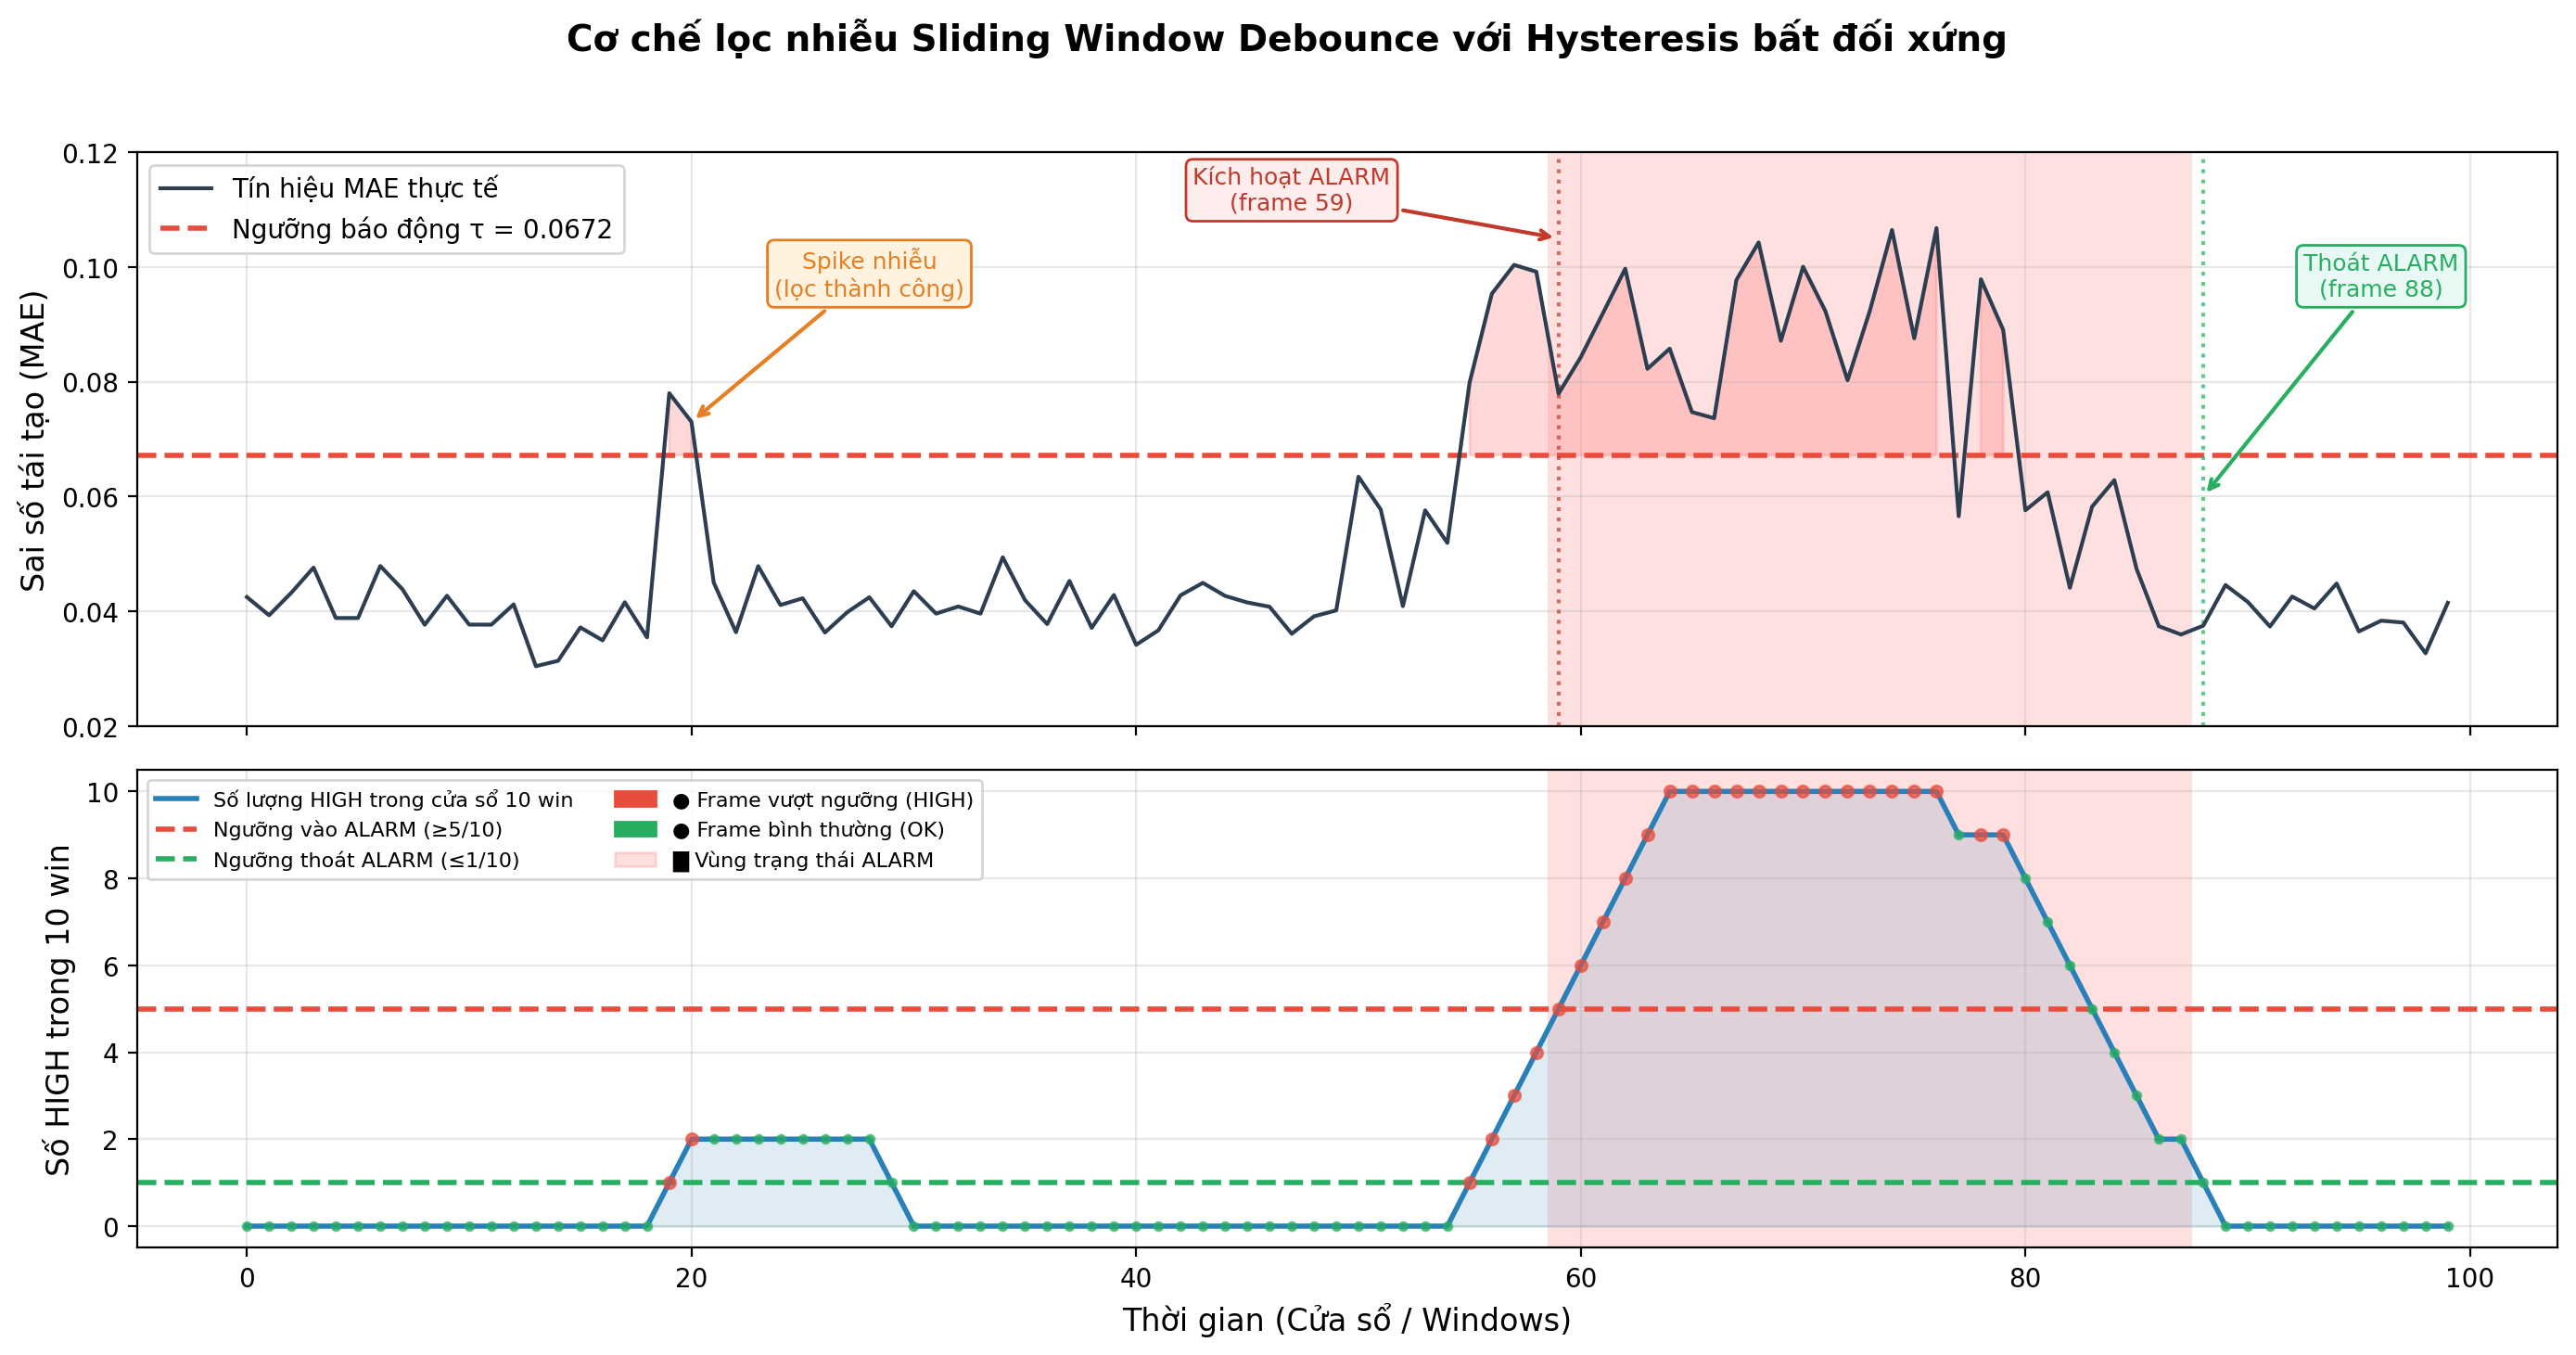
\includegraphics[width=0.95\linewidth]{chap4/image/debounce_sliding_window.png}
    \caption[Cơ chế lọc nhiễu bằng cửa sổ trượt]{Mô phỏng cơ chế cửa sổ trượt kết hợp trễ bất đối xứng: kích hoạt cảnh báo khi $\geq 5/10$ mẫu vượt ngưỡng, phục hồi khi $\leq 1/10$ mẫu vượt ngưỡng. Xung nhiễu đơn lẻ (frame 19--21) được lọc hoàn toàn nhờ cơ chế biểu quyết đa số.}
    \label{fig:debounce_logic}
\end{figure}

Kỹ thuật lọc trễ phần mềm này hoạt động như bộ lọc thông thấp cho logic quyết định, loại bỏ các đỉnh nhiễu ngẫu nhiên và giúp hệ thống đạt độ tin cậy cực cao (F1-Score $> 0{,}98$) trong các bài kiểm tra thực địa dài hạn.
